\documentclass{article}
\usepackage{amsmath}
\usepackage{amsthm}
\usepackage{amssymb}
\usepackage{dirtytalk}
\usepackage{enumerate}
\usepackage[margin=1.00in]{geometry}
\usepackage{graphicx}
\usepackage{hyperref}
\usepackage{tikz}

% define colors
\definecolor{white}{RGB}{255,255,255} % white
\definecolor{gray}{RGB}{192,192,192} % gray
\definecolor{black}{RGB}{0,0,0} % black
\definecolor{sky_blue}{RGB}{135,206,250} % sky blue

% new theorems and definitions
\newtheorem{theorem}{Theorem}[section]
\newtheorem{proposition}[theorem]{Proposition}
\newtheorem{corollary}[theorem]{Corollary}
\newtheorem{lemma}[theorem]{Lemma}
\newtheorem{question}[theorem]{Question}
\theoremstyle{definition}
\newtheorem{remark}[theorem]{Remark}

% new commands and math operators
\newcommand\abs[1]{\left|#1\right|}
\newcommand\nullity[1]{\operatorname{nullity}\left(#1\right)}
\newcommand\kernel[1]{\operatorname{null}\left(#1\right)}
\newcommand\rank[1]{\operatorname{rank}\left(#1\right)}

\title{On Zero Forcing and the Inverse Eigenvalue Problem for Graphs}
\author{Thomas R. Cameron}
\date{\today}

\begin{document}
\maketitle
\abstract{This note is intended to introduce the connection between the inverse eigenvalue problem of a graph and the zero forcing number of a graph.}
%%%%%%%%%%%%%%%%%%%%%%%%%%%%%%%%%%%%%%%%%%%%%%%%%%%%%%
%                                    				Introduction
%%%%%%%%%%%%%%%%%%%%%%%%%%%%%%%%%%%%%%%%%%%%%%%%%%%%%%
\section{Introduction}	\label{sec:intro}
Let $\mathbb{G}$ denote the collection of all simple graphs (no loops nor multi-edges) of order $n$.
With each graph $G\in\mathbb{G}$, there is a vertex set $V(G) = \{v_{1},v_{2},\ldots,v_{n}\}$ and an edge set $E(G)$, where $\{v_{i},v_{j}\}\in E(G)$ if and only if $i\neq j$ and $v_{i}$ and $v_{j}$ are adjacent vertices.
For example, let $G$ be the star graph of order $7$ shown in Figure~\ref{fig:star-graph}.
Then, $V(G) = \{1,2,3,4,5,6,7\}$ and $E(G) = \{\{1,7\},\{2,7\},\{3,7\},\{4,7\},\{5,7\},\{6,7\}\}$. 

%%%%%%%%%%%%%%%%
%					Figure 1				%
%%%%%%%%%%%%%%%%
\begin{figure}[ht]
\centering
\resizebox{0.20\textwidth}{!}{% Star Graph
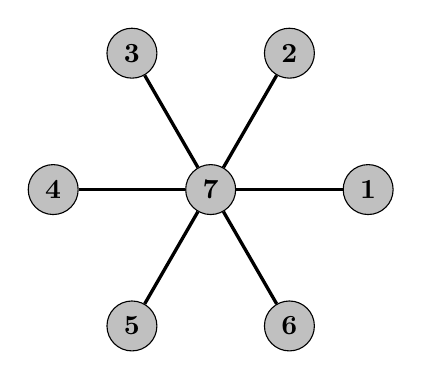
\begin{tikzpicture}
	\node[circle,draw=black,fill=gray] (1) at (2,0) {\textbf{1}};
	\node[circle,draw=black,fill=gray] (2) at (1,1.732) {\textbf{2}};
	\node[circle,draw=black,fill=gray] (3) at (-1,1.732) {\textbf{3}};
	\node[circle,draw=black,fill=gray] (4) at (-2,0) {\textbf{4}};
	\node[circle,draw=black,fill=gray] (5) at (-1,-1.732) {\textbf{5}};
	\node[circle,draw=black,fill=gray] (6) at (1,-1.732) {\textbf{6}};
	\node[circle,draw=black,fill=gray] (7) at (0,0) {\textbf{7}};
	
	\foreach \x/\y in {7/1,7/2,7/3,7/4,7/5,7/6}
		\draw[black,=>latex',very thick] (\x) -- (\y);
\end{tikzpicture}%
}
\caption{A star graph of order $7$.}
\label{fig:star-graph}
\end{figure}

Every $n\times n$ symmetric matrix $A=[a_{ij}]_{i,j=1}^{n}$ is associated with a graph $G\in\mathbb{G}$, where $a_{ij}\neq 0$ if and only if $\{v_{i},v_{j}\}\in E(G)$.
Given a graph $G\in\mathbb{G}$, the set of all $n\times n$ symmetric matrices associated with $G$ is denoted by
\[
\mathcal{S}(G) = \left\{A=[a_{ij}]_{i,j=1}^{n}\colon a_{ij}=a_{ji}~\forall i\neq j,~a_{ij}\neq 0~\Leftrightarrow~\{v_{i},v_{j}\}\in E(G)\right\}.
\]
For example, the star graph $G$ shown in Figure~\ref{fig:star-graph} is associated with symmetric matrices of the form
\[
A = \begin{bmatrix} 
		\alpha_{1} & 0 & \cdots & 0 & \beta_{1} \\
		0 & \alpha_{2} & \cdots & 0 & \beta_{2} \\
		\vdots & & \ddots & &  \vdots \\
		0 & & & \alpha_{6} & \beta_{6} \\
		\beta_{1} & \beta_{2} & \cdots & \beta_{6} & \alpha_{7} \\
	\end{bmatrix}.
\]

The inverse eigenvalue problem of a graph can be stated as follows:
Given a graph $G\in\mathbb{G}$, what are all possible length $n$ multi-sets $\sigma$ such that there is a matrix $A\in\mathcal{S}(G)$ with spectrum $\sigma$.
This important question is obviously difficult to answer in general; however, there are a few observations we can make. 
\begin{itemize}
\item  The empty graph of order $n$, denoted $E_{n}$, has no edges.
		Therefore, $\mathcal{S}(E_{n})$ is the set of all $n\times n$ diagonal matrices.
		Since the eigenvalues of a diagonal matrix are equal to its diagonal entries, it follows that every length $n$ multi-set $\sigma$ corresponds to the eigenvalues of a matrix $A\in\mathcal{S}(E_{n})$.
		It turns out, that the empty graph is the only graph with this property. 
\item Let $K_{n}$ denote a complete graph of order $n$.
		Then, $\mathcal{S}(K_{n})$ is made up of symmetric matrices where all off-diagonal entries are non-zero. 
		Furthermore, for any $\lambda_{1}\leq\lambda_{2}\leq\cdots\lambda_{n}$, there is a matrix $A\in\mathcal{S}(K_{n})$ with eigenvalues $\lambda_{1},\lambda_{2},\ldots,\lambda_{n}$ if and only if $\lambda_{1}<\lambda_{n}$~\cite{Barrett2013}.
\item Let $P_{n}$ denote a path graph of order $n$.
		Then, $\mathcal{S}(P_{n})$ corresponds to tri-diagonal matrices with non-zero entries in the upper and lower diagonals.
		Furthermore, any length $n$ multi-set $\sigma$ corresponds to the eigenvalues of a matrix $A\in\mathcal{S}(P_{n})$ if and only if the entries of $\sigma$ are distinct~\cite{Hochstadt1967}.
\end{itemize}

Due to the difficulty of the inverse eigenvalue problem of a graph, there is a focus on solving related but seemingly easier problems.
For instance, one may want to find the maximum multiplicity of a graph $G\in\mathbb{G}$, denoted $M(G)$, which is defined as the largest integer $k$ such that there is a matrix $A\in\mathcal{S}(G)$ with an eigenvalue of multiplicity $k$.
Note $M(E_{n})=n$, $M(K_{n})=(n-1)$,  and $M(P_{n})=1$.

The multiplicity of an eigenvalue $\lambda$ of the symmetric matrix $A$ is equal to the nullity of $\lambda I - A$, i.e,  the dimension of the null space of $\lambda I-A$.
Note that for any $A\in\mathcal{S}(G)$, it follows that $\lambda I - A\in\mathcal{S}(G)$.
Therefore,
\[
M(G) = \max\left\{\nullity{A}\colon A\in\mathcal{S}(G)\right\}.
\]
For this reason, the maximum multiplicity of a graph is often refereed to as the max nullity of the graph. 

In a similar manner, the minimum rank of $G$, denoted $mr(G)$, is defined by 
\[
mr(G) = \min\left\{\rank{A}\colon A\in\mathcal{S}(G)\right\}.
\]
Recall that the $\rank{A}$ is the dimension of the column space of $A$.
By the rank-nullity theorem, we have
\[
mr(G) + M(G) = n.
\]

In 2006, at the AIMS Workshop on \say{Spectra of families of matrices described by graphs, digraphs, and sign pattern}, a novel connection between the maximum nullity of a graph and its zero forcing number was presented. 
Zero forcing was introduced independently by Burgarth and Giovannetti in the control of quantum systems~\cite{Burgarth2007}, where it was called graph infection.
For our purposes, zero forcing is a coloring game on a graph, where an initial set of vertices are colored blue and all other vertices are colored white.
Then, the blue vertices force neighboring white vertices blue using a color change rule.
There are many color changing rules, but the standard rule is that a blue vertex $b$ can force a white vertex $w$ blue if $w$ is the only white neighbor of $b$.
We will reference this rule as the Z-color change rule to distinguish it from the other variants. 

Given a  graph $G\in\mathbb{G}$, let $B\subseteq V(G)$ denote the initial set of blue vertices; this is called the initial coloring of $G$.
Then, denote by $B^{[t]}$ the blue vertices after $t$ applications of the Z-color change rule, where $B^{[0]}=B$.
Because the graph is finite, there exists a $t^{*}\geq 0$ for which $B^{[t^{*}]} = B^{[t^{*}+k]}$, for all $k\in\mathbb{N}$, i.e., no more changes are possible from applying the Z-color change rule. 
We reference $B^{[t^{*}]}$ as the final coloring of $B$.
If $B^{[t^{*}]} = V(G)$, i.e., the final coloring is all of the vertices of $G$, then we say that $B$ is a zero forcing set of $G$.
The zero forcing number of $G$ is defined as the cardinality of the smallest zero forcing set of $G$:
\[
Z(G) = \min\left\{\abs{B}\colon B^{[t^{*}]} = V(G)\right\}.
\]

For example, consider the application of the Z-color change rule to a path graph on $5$ vertices shown in Figure~\ref{fig:path-graph-coloring}.
It is clear that $B^{[4]}$ is the final coloring of $B$ since $B^{[5]} = B^{[4]}$.
Furthermore, since $B^{[4]}$ encompasses all vertices in the graph, it follows that $B=\{1\}$ is a zero forcing set and, hence, the zero forcing number of this path graph is equal to $1$.
%%%%%%%%%%%%%%%%
%					Figure 2			%
%%%%%%%%%%%%%%%%
\begin{figure}[ht]
\centering
\resizebox{0.75\textwidth}{!}{% Path Graph Coloring
\begin{tabular}{ccc}
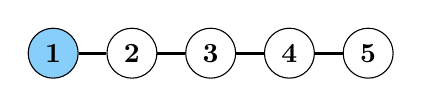
\begin{tikzpicture}
	\node[circle,draw=black,fill=sky_blue] (1) at (-2,0) {\textbf{1}};
	\node[circle,draw=black,fill=white] (2) at (-1,0) {\textbf{2}};
	\node[circle,draw=black,fill=white] (3) at (0,0) {\textbf{3}};
	\node[circle,draw=black,fill=white] (4) at (1,0) {\textbf{4}};
	\node[circle,draw=black,fill=white] (5) at (2,0) {\textbf{5}};
	
	\foreach \x/\y in {1/2,2/3,3/4,4/5}
		\draw[black,=>latex',very thick] (\x) -- (\y);
\end{tikzpicture}
&
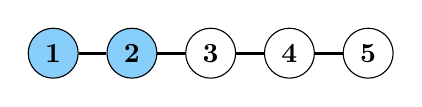
\begin{tikzpicture}
	\node[circle,draw=black,fill=sky_blue] (1) at (-2,0) {\textbf{1}};
	\node[circle,draw=black,fill=sky_blue] (2) at (-1,0) {\textbf{2}};
	\node[circle,draw=black,fill=white] (3) at (0,0) {\textbf{3}};
	\node[circle,draw=black,fill=white] (4) at (1,0) {\textbf{4}};
	\node[circle,draw=black,fill=white] (5) at (2,0) {\textbf{5}};
	
	\foreach \x/\y in {1/2,2/3,3/4,4/5}
		\draw[black,=>latex',very thick] (\x) -- (\y);
\end{tikzpicture}
&
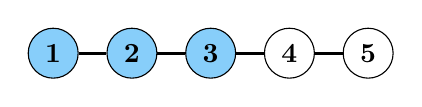
\begin{tikzpicture}
	\node[circle,draw=black,fill=sky_blue] (1) at (-2,0) {\textbf{1}};
	\node[circle,draw=black,fill=sky_blue] (2) at (-1,0) {\textbf{2}};
	\node[circle,draw=black,fill=sky_blue] (3) at (0,0) {\textbf{3}};
	\node[circle,draw=black,fill=white] (4) at (1,0) {\textbf{4}};
	\node[circle,draw=black,fill=white] (5) at (2,0) {\textbf{5}};
	
	\foreach \x/\y in {1/2,2/3,3/4,4/5}
		\draw[black,=>latex',very thick] (\x) -- (\y);
\end{tikzpicture}
\\ $B^{[0]} = \{1\}$ & $B^{[1]} = \{1,2\}$ & $B^{[2]} = \{1,2,3\}$ \\
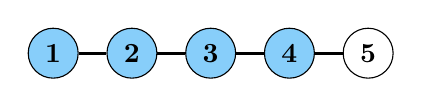
\begin{tikzpicture}
	\node[circle,draw=black,fill=sky_blue] (1) at (-2,0) {\textbf{1}};
	\node[circle,draw=black,fill=sky_blue] (2) at (-1,0) {\textbf{2}};
	\node[circle,draw=black,fill=sky_blue] (3) at (0,0) {\textbf{3}};
	\node[circle,draw=black,fill=sky_blue] (4) at (1,0) {\textbf{4}};
	\node[circle,draw=black,fill=white] (5) at (2,0) {\textbf{5}};
	
	\foreach \x/\y in {1/2,2/3,3/4,4/5}
		\draw[black,=>latex',very thick] (\x) -- (\y);
\end{tikzpicture}
&
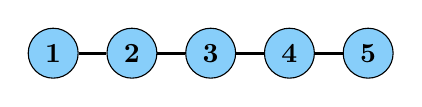
\begin{tikzpicture}
	\node[circle,draw=black,fill=sky_blue] (1) at (-2,0) {\textbf{1}};
	\node[circle,draw=black,fill=sky_blue] (2) at (-1,0) {\textbf{2}};
	\node[circle,draw=black,fill=sky_blue] (3) at (0,0) {\textbf{3}};
	\node[circle,draw=black,fill=sky_blue] (4) at (1,0) {\textbf{4}};
	\node[circle,draw=black,fill=sky_blue] (5) at (2,0) {\textbf{5}};
	
	\foreach \x/\y in {1/2,2/3,3/4,4/5}
		\draw[black,=>latex',very thick] (\x) -- (\y);
\end{tikzpicture}
&
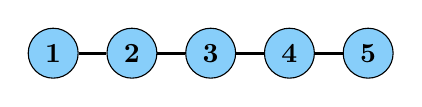
\begin{tikzpicture}
	\node[circle,draw=black,fill=sky_blue] (1) at (-2,0) {\textbf{1}};
	\node[circle,draw=black,fill=sky_blue] (2) at (-1,0) {\textbf{2}};
	\node[circle,draw=black,fill=sky_blue] (3) at (0,0) {\textbf{3}};
	\node[circle,draw=black,fill=sky_blue] (4) at (1,0) {\textbf{4}};
	\node[circle,draw=black,fill=sky_blue] (5) at (2,0) {\textbf{5}};
	
	\foreach \x/\y in {1/2,2/3,3/4,4/5}
		\draw[black,=>latex',very thick] (\x) -- (\y);
\end{tikzpicture}
\\ $B^{[3]} = \{1,2,3,4\}$ & $B^{[4]} = \{1,2,3,4,5\}$ & $B^{[5]} = \{1,2,3,4,5\}$ \\
\end{tabular}%
}
\caption{A zero forcing set for a path graph of order $5$.}
\label{fig:path-graph-coloring}
\end{figure}

One can easily generalize the above example and conclude that the zero forcing number of all path graphs is equal to $1$, i.e., $Z(P_{n}) = 1$.
Note that not every initial coloring of $1$ vertex is a zero forcing set of $P_{n}$. 
Indeed, consider the initial coloring of a path graph on $5$ vertices shown in Figure~\ref{fig:path-graph-coloring2}.

%%%%%%%%%%%%%%%%
%					Figure 3			%
%%%%%%%%%%%%%%%%
\begin{figure}[ht]
\centering
\resizebox{0.25\textwidth}{!}{% Path Graph Coloring 2
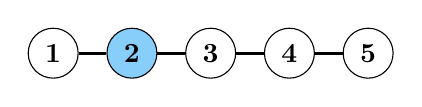
\begin{tikzpicture}
	\node[circle,draw=black,fill=white] (1) at (-2,0) {\textbf{1}};
	\node[circle,draw=black,fill=sky_blue] (2) at (-1,0) {\textbf{2}};
	\node[circle,draw=black,fill=white] (3) at (0,0) {\textbf{3}};
	\node[circle,draw=black,fill=white] (4) at (1,0) {\textbf{4}};
	\node[circle,draw=black,fill=white] (5) at (2,0) {\textbf{5}};
	
	\foreach \x/\y in {1/2,2/3,3/4,4/5}
		\draw[black,=>latex',very thick] (\x) -- (\y);
\end{tikzpicture}%
}
\caption{A non zero forcing set for a path graph of order $5$.}
\label{fig:path-graph-coloring2}
\end{figure}

We are now ready to present the connection between the zero forcing number and the maximum nullity of a graph.
First we require the following lemma. 
%%%%%%%%%%%%%%%%
%					Lemma 1.1			%
%%%%%%%%%%%%%%%%
\begin{lemma}\label{lem:non-zero-int}
Suppose that $\alpha\subseteq\{1,2,\ldots,n\}$ with $\abs{\alpha}<k$ and $U$ is a subspace of $\mathbb{R}^{n}$ of dimension $k$.
Then, $U$ contains a non-zero vector of $\textbf{v}$ with $\textbf{v}[\alpha] = 0$.
\end{lemma}
\begin{proof}
Note that if $U$ and $V$ are subspaces of $\mathbb{R}^{n}$ whose dimensions satisfy
\[
\dim{V} > n - \dim{U},
\]
then $U$ and $V$ must have a non-trivial intersection, i.e., there is a non-zero vector in $U\cap V$.
Now, define
\[
V = \left\{\textbf{v}\in\mathbb{R}^{n}\colon \textbf{v}[\alpha] = 0\right\},
\]
and note that $\dim{V} = n - \abs{\alpha} > n - k = \dim{U}$.
Hence, there exists a non-zero vector $\textbf{v}\in U\cap V$, and the result follows.
\end{proof}

%%%%%%%%%%%%%%%%
%					Theorem 1.2		%
%%%%%%%%%%%%%%%%
\begin{theorem}\label{thm:max-nul-zero-forcing}
Let $G\in\mathbb{G}$.
Then, $M(G)\leq Z(G)$.
\end{theorem}
\begin{proof}
Let $B\subseteq V(G)$ be a zero forcing set of $G$, and let $A\in\mathcal{S}(G)$.
If $\abs{B}<\nullity{A}$, then Lemma~\ref{lem:non-zero-int} implies that there exists a non-zero vector $\textbf{x}\in\kernel{A}$ such that $\textbf{x}_{i}=0$ for all $i\in B$.
However, if a vector $\textbf{x}\in\kernel{A}$ satisfies $\textbf{x}_{i}=0$ for all $i\in B$, then it follows that $\textbf{x}=\textbf{0}$.

Indeed, let $j\in V(G)\setminus{B}$ be any vertex that is forced by some $i\in B$; at least one such vertex must exist since $B$ is a zero forcing set.
Then, the equation $A\textbf{x}=\textbf{0}$ implies that $a_{ij}\textbf{x}_{j}=0$, which gives $\textbf{x}_{j}=0$ since $a_{ij}\neq 0$.
If necessary, we can repeat the above argument on the zero forcing set $B\cup\{j\}$, and perhaps again, until all vertices in $V(G)$ are accounted for at which point it follows that $\textbf{x}=\textbf{0}$.

This contradiction with Lemma~\ref{lem:non-zero-int} implies that $\abs{B}\geq\nullity{A}$.
Since $B$ and $A$ are arbitrary, it follows that $Z(G)\geq M(G)$.
\end{proof}

Theorem~\ref{thm:max-nul-zero-forcing} can be used to determine the maximum nullity of a graph via its zero forcing number. 
For instance, we know that the path graph satisfies $Z(P_{n})=1$.
Therefore, Theorem~\ref{thm:max-nul-zero-forcing} implies that $M(P_{n}) \leq 1$.
Since there is always a singular matrix in $\mathcal{S}(G)$, for any graph $G$, it follows that $M(P_{n})=1$.

As a more interesting example, consider the star graph in Figure~\ref{fig:star-graph}.
Note that $B=\{1,2,3,4,5\}$ is a zero-forcing set of minimal size. 
This observation can easily be generalized and we conclude that the zero forcing number of the star graph $K_{1,n-1}$ of order $n$ satisfies $Z(K_{1,n-1}) = n-2$.
Therefore, the maximum nullity and minimum rank satisfy
\[
M(K_{1,n-1}) \leq n-2~\text{and}~mr(K_{1,n-1}) \geq 2,
\]
respectively.
Furthermore, the adjacency matrix of the star graph $K_{1,n-1}$:
\[
A = \begin{bmatrix} 
		0 & 0 & \cdots & 0 & 1 \\
		0 & 0 & \cdots & 0 & 1 \\
		\vdots & & \ddots & &  \vdots \\
		0 & & & 0 & 1 \\
		1 & 1 & \cdots & 1 & 0 \\
	\end{bmatrix}.
\]
is a $n\times n$ matrix in $\mathcal{S}(K_{1,n-1})$ that satisfies $\rank{A} = 2$.
Therefore, $M(K_{1,n-1})=n-2$ and $mr(K_{1,n-2}) = 2$.

%%%%%%%%%%%%%%%%%%%%%%%%%%%%%%%%%%%%%%%%%%%%%%%%%%%%%%
%                                    				Positive Semidefinite Zero Forcing
%%%%%%%%%%%%%%%%%%%%%%%%%%%%%%%%%%%%%%%%%%%%%%%%%%%%%%
\section{Positive Semidefinite Zero Forcing}\label{sec:psd-zf}
As mentioned in Section~\ref{sec:intro}, there are many color change rules that can be used in the coloring game of zero forcing. 
The so-called standard zero forcing rule provides an upper bound on the maximum nullity of a graph via Theorem~\ref{thm:max-nul-zero-forcing}.
The positive semidefinite zero forcing rule provides an upper bound on the maximum positive semidefinite nullity:
\[
M_{+}(G) = \max\left\{\nullity{A}\colon A\in S(G),~\forall\lambda\in\sigma(A),~\lambda\geq 0\right\}.
\]
Note that the additional condition on the eigenvalues of $A$, i.e., $\lambda\geq 0$ for all $\lambda\in\sigma(A)$, implies that $A$ must be positive semidefinite. 
%Furthermore, because the eigenvalues must be non-negative, $M_{+}(G)$ no longer corresponds to the maximum multiplicity of an eigenvalue of a positive semidefinite matrix in $\mathcal{S}(G)$.

Given a graph $G\in\mathbb{G}$, let $B\subseteq V(G)$ denote the initial coloring of $G$. 
Let $G\setminus{B}$ denote the resulting graph after the blue vertices (and adjacent edges) have been removed, and let $W_{1},\ldots,W_{k}$ denote the vertex sets of the connected components of $G-B$.
If $b\in B$ and $w\in W_{i}$ is the only white neighbor of $b$ in $G[W_{i}\cup B]$, for some $i\in\{1,\ldots,k\}$, then the positive semidefinite zero forcing rule says that $b$ can force $w$ blue.

As with the standard zero forcing rule, there exists a $t^{*}\geq 0$ such that $B^{[t^{*}]} = B^{[t^{*}+k]}$ for all $k\in\mathbb{N}$, and we say that $B$ is a positive semidefinite zero forcing set if the final coloring satisfies $B^{[t^{*}]} = V(G)$.
The positive semidefinite zero forcing number of $G$ is defined as the cardinality of the smallest positive semidefinite zero forcing set of $G$:
\[
Z_{+}(G) = \min\left\{\abs{B}\colon B^{[t^{*}]} = V(G)\right\}.
\]
%%%%%%%%%%%%%%%%
%					Theorem 2.1		%
%%%%%%%%%%%%%%%%
\begin{theorem}\label{thm:psd-max-nul-zero-forcing}
Let $G\in\mathbb{G}$.
Then, $M_{+}(G)\leq Z_{+}(G)$.
\end{theorem}
\begin{proof}
Let $A\in S(G)$ be positive semidefinite with $\nullity{A}=M_{+}(G)$ and consider a non-zero vector $\textbf{x}\in\null{A}$, which is guaranteed to exist since the max nullity is at least $1$.
Let $B\subset V(G)$ denote the set of vertices such that $\textbf{x}_{i}=0$, and let $W_{1},\ldots,W_{k}$ denote the vertex sets of the connected components of $G\setminus{B}$.
For every $i\in\{1,\ldots,k\}$, we claim that no $w\in W_{i}$ can be the only neighbor of a $b\in B$ in $G[W_{i}\cup B]$.

Indeed, note that we can write $A$, possibly after re-ordering the vertices of $G$, as follows 
\[
A = \begin{bmatrix}
		A_{1} & 0 & \cdots & 0 & C_{1} \\
		0 & A_{2} & \cdots & 0 & C_{2} \\
		\vdots & \vdots & \ddots & \vdots & \vdots \\
		0 & 0 & \cdots & A_{k} & C_{k} \\
		C_{1} & C_{2} & \cdots & C_{k} & D \\
		\end{bmatrix},
\]
where $A_{1},\ldots,A_{k}$ corresponds to the vertex sets $W_{1},\ldots,W_{k}$, respectively, $D$ corresponds to the vertex set $B$, and $C_{i}$ corresponds to the edges between $W_{i}$ and $B$, for all $i\in\{1,\ldots,k\}$.

Now, consider the partition $\textbf{x} = [\textbf{x}_{1}^{T},\ldots,\textbf{x}_{k}^{T},\textbf{0}^{T}]$, where $\textbf{x}_{i}$ has size equal to $\abs{W_{i}}$, for all $i\in\{1,\ldots,k\}$, and the zero vector $\textbf{0}$ has size equal to $\abs{B}$.
Note that all entries of $\textbf{x}_{1},\ldots,\textbf{x}_{k}$ must be non-zero.
Moreover, the equation $A\textbf{x}=\textbf{0}$ implies that $A_{i}\textbf{x}_{i}=\textbf{0}$ for all $i\in\{1,\ldots,k\}$.

The column inclusion property for Hermitian positive semidefinite matrices~\cite{Johnson1998}, guarantees that each column in $C_{i}$ is the span of the columns in $A_{i}$, for all $i\in\{1,\ldots,k\}$.
Therefore, for each $i\in\{1,\ldots,k\}$, there exists a matrix $Y_{i}$ such that $C_{i}=A_{i}Y_{i}$.
Since $A$ is symmetric, it follows that $C_{i}=Y_{i}^{T}A_{i}$; hence, $C_{i}\textbf{x}_{i}=\textbf{0}$ for all $i\in\{1,\ldots,k\}$.
But if $w\in W_{i}$ were the only white neighbor of $b\in B$ in $G[W_{i}\cup B]$, then $C_{i}\textbf{x}_{i}\neq \textbf{0}$, which is a contradiction. 

This contradiction implies that $B$ is not a positive semidefinite zero forcing set of $G$.
Furthermore, it follows that there is no non-trivial $\textbf{x}\in\kernel{A}$ with $\textbf{x}_{i}=0$ for all $i$ in a positive semidefinite zero forcing set of $G$.
Therefore, by Lemma~\ref{lem:non-zero-int}, we have $M_{+}(G)\leq Z_{+}(G)$.
\end{proof}

As an example of how Theorem~\ref{thm:psd-max-nul-zero-forcing} could be applied, consider the star graph $K_{1,n-1}$. 
Note that the \say{center} vertex constitutes a positive semidefinite zero forcing set of $K_{1,n-1}$.
Therefore, 
\[
Z_{+}(K_{1,n-1}) = 1
\]
and it follows that $M_{+}(K_{1,n-1}) = 1$.

Finally, note that every standard zero forcing set of a graph $G\in\mathbb{G}$ constitutes a positive semidefinite zero forcing set; hence, $Z_{+}(G)\leq Z(G)$.
Furthermore, it is also clear that $M_{+}(G)\leq M(G)$.
%%%%%%%%%%%%%%%%
%					Question 2.2		%
%%%%%%%%%%%%%%%%
\begin{question}
Is there a relationship between $Z_{+}(G)$ and $M(G)$, i.e., does the following hold
\[
Z_{+}(G) \leq M(G)
\]
for all (or some) graphs $G\in\mathbb{G}$.
\end{question}

%%%%%%%%%%%%%%%%%%%%%%%%%%%%%%%%%%%%%%%%%%%%%%%%%%%%%%
%								Computation of Max Nullity and Zero-Forcing
%%%%%%%%%%%%%%%%%%%%%%%%%%%%%%%%%%%%%%%%%%%%%%%%%%%%%%
\section{Computation of Max Nullity and Zero-Forcing}
%%%%%%%%%%%%%%%%%%%%%%%%%%%%%%%%%%%%%%%%%%%%%%%%%%%%%%
%								Colin de Verdi{\'e}re Type Parameters
%%%%%%%%%%%%%%%%%%%%%%%%%%%%%%%%%%%%%%%%%%%%%%%%%%%%%%
\section{Colin de Verdi{\'e}re Type Parameters}
%%%%%%%%%%%%%%%%%%%%%%%%%%%%%%%%%%%%%%%%%%%%%%%%%%%%%%
%                                 	   			Bibliography
%%%%%%%%%%%%%%%%%%%%%%%%%%%%%%%%%%%%%%%%%%%%%%%%%%%%%%
\label{Bibliography}
\bibliographystyle{siam}
\bibliography{Bibliography}

\end{document}